\section{Linearisieren}
\subsection{Vereinfachung des Modells (virtell)}
Diese Linearisierung wird verwendet, wenn die Nichtlinearitäten nicht allzu gravierend sind. Also beispielsweise wenn Kennlinien nicht stark gekrümmt sind etc. Bei dieser Methoden werden alle nicht linearen Blöck am Arbeitspunkt linearisiert \script{93}. Gegebenfalls muss ein Feedforward-Path implementiert werden, um Sicherzustellen, dass ein Regler nur am Arbeitspunkt arbeitet.
\begin{center}
	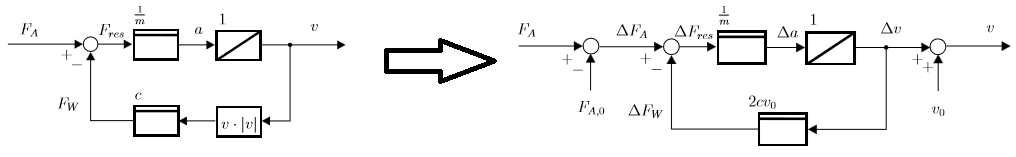
\includegraphics[width=\columnwidth]{Images/virtuell_linearisierung}
\end{center}


\subsection{Veränderung der Strecke (konstruktiv)}
Wenn eine Inverse Funktion vor der Regelstrecke implementiert wird, wird ein Teil der Strecke übersprungen. Das bedeutet, dass zB ein Input $\tilde{u}$ direkt bei $w$ eingefügt wird ($w = \tilde{u}$) was die Nicht-Linearität aufheben kann, sofern $f^{-1}$ existiert und genügend genau ist.\script{95}
\begin{center}
	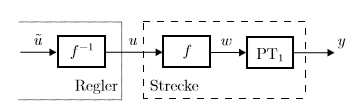
\includegraphics[width=0.6\columnwidth]{Images/konstruktiv_linearisierung}
\end{center}


\subsection{Mathematische Formulierungen}
\subsubsection{Taylor-Reihe}
Wenn eine Funktion Linearisiert werden muss, kann das erste Glied der Tayler-Reihe verwendet werden. Dabei ist die Taylor-Reihe mit Entwicklungsstelle $x_0$
\[
T_{f(x),x_0} = \sum_{n=0}^{\infty}\frac{f^{(n)}(x_0)}{n!}(x-x_0)^n
\]

\noindent\textbf{Beispiel:}
\begin{align*}
	T_{\sin(x), x_0 = 0} &= \overbrace{\frac{\cos(0)}{0!}(x - 0)^1}^{\text{Glied 1.}} + \overbrace{\frac{-\cos(0)}{3!}(x - 0)^3}^{\text{Glied 3.}} + \cdots \\
	&= x - \frac{x^3}{3!} + \cdots
\end{align*}

\noindent Wichtigste Linearisierungen
\begin{align*}
	\sin(x) &\approxeq x \\
	\cos(x) &\approxeq 1 \\
	\tan(x) &\approxeq x \\
	e^x &\approxeq 1 + x \\
	\ln(1 + x) &\approxeq x \qquad\qquad\in(-1;1]
\end{align*}


\subsubsection{Least Square}
Findet eine Gerade welche die Varianz, Quadratischer Abstand von Gerade, minimiert. 
\begin{center}
	\begin{minipage}{0.20\textwidth}
		\begin{center}
			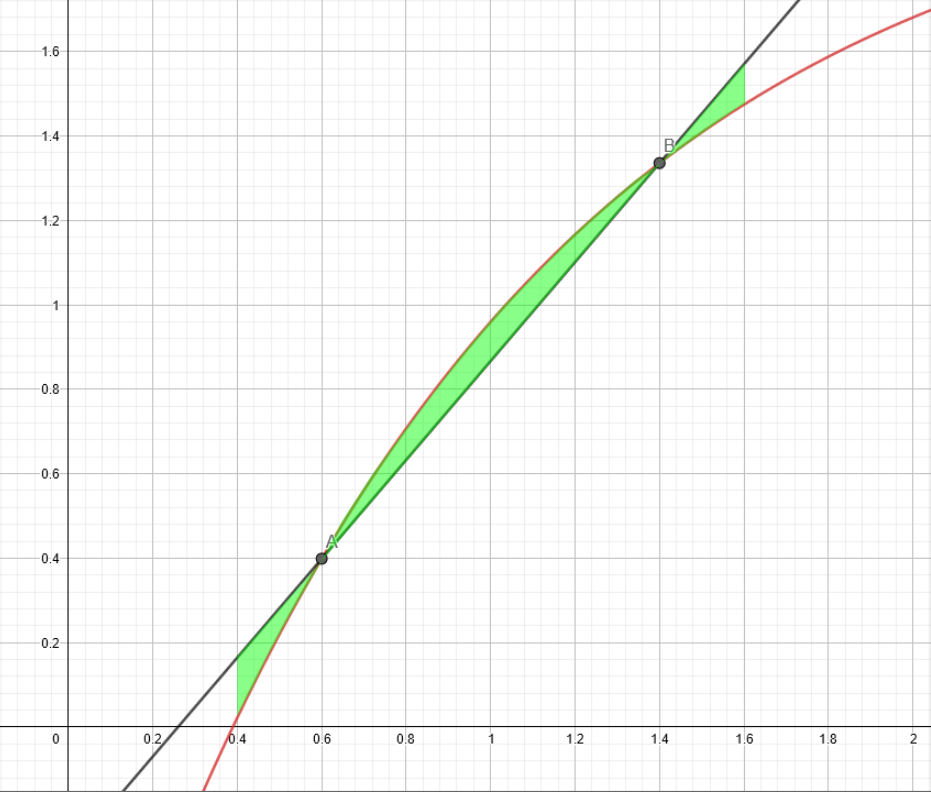
\includegraphics[width=\linewidth,keepaspectratio=true]{Images/leastsquare}\\
		\end{center}
	\end{minipage}%%% to prevent a space
	\begin{minipage}{0.3\textwidth}
		\[\textcolor{red}{\vec{x}} = (A^TA)^{-1}A^T\vec{b}\]
	\end{minipage}
\end{center}

\noindent
Beispiel für \textbf{streng Lineares System} ($b=0$): $y_i = \textcolor{red}{a}x_i$.
\[
\underbrace{\begin{pmatrix}
		x_1 \\
		x_2 \\
		\vdots \\
		x_n
\end{pmatrix}}_{\scriptsize{A}}
\cdot
\underbrace{\begin{pmatrix}
		\textcolor{red}{a}
\end{pmatrix}}_{\scriptsize{\textcolor{red}{\vec{x}}}}
=
\underbrace{\begin{pmatrix}
		y_1 \\
		y_2 \\
		\vdots \\
		y_n
\end{pmatrix}}_{\scriptsize{\vec{b}}}
\]

\noindent Für $y = ax$ gilt $P_1 = (1, 40), P_2 = (2,70)$ gilt:
\begin{align*}
	a = \left(\underbrace{\begin{bmatrix} 1 & 2 \end{bmatrix}\begin{bmatrix} 1 \\ 2 \end{bmatrix}}_{5}\right)^{-1}\underbrace{\begin{bmatrix} 1 & 2 \end{bmatrix}\begin{bmatrix} 40 \\ 70 \end{bmatrix}}_{180} = 36
\end{align*}